\chapter{Motivación y Antecedentes}
\section{Crecimiento de la red}
El gran crecimiento en la cantidad de sistemas teconológicos interconectados via Internet en el mundo en los últimos 30 años es algo que no ha dejado indiferente a nadie. Para entender este fenómeno, distintos organismos internacionales se dedican periodicamente a realizar estimaciones de dicha cifra. Un caso muy popular de dicha labor es el contador global de conexiones móviles a Internet del GSMA Intelligence\footnote{\url{https://gsmaintelligence.com/}} el cual recientemente ha estimado en más de 7 mil millones el número de dispositivos móviles con conexión a la red, superando por primera vez al total de la población mundial\footnote{\url{http://www.cnet.com/news/there-are-now-more-gadgets-on-earth-than-people/}}. Una premisa que coincide con el último informe \emph{The State Of Internet} de \emph{Akamai} \cite{report:akamai} donde se resume el estudio de las principales variaciones en capacidad de acceso, velocidades de acceso, tipos de ataques, etc. a Internet de que disponen distintos países del mundo. Éste estudio corroboró lo que ya ha sido tendencia en los últimos años: Tanto las velocidades de navegación, así como el total de conexiones a Internet han aumentado generalizadamente en todo el planeta. Las proyecciones a futuro preservan ésta tendencia apostando a que tanto la cantidad de dispositivos como el número de accesos a Internet deberían seguir subiendo \cite{nota:2020}, ello producto de factores como la reducción de costos de producción y la minimización de la tecnología, además de distintas tendencias generadas a raíz del fenómeno de \emph{globalización} que -en gran medida- nos ha forzado a participar de una sociedad más interconectada en todo el mundo y explicarían dicha tendencia. Olvidando un poco las interpretaciones o justificaciones para ésta situación, el hecho concreto es que existe una directa proporcionalidad entre el número de dispositivos y los requerimientos de accesos a la red, y hoy ambos están en su apogeo de crecimiento.

\begin{figure}[!h]
	\centering
	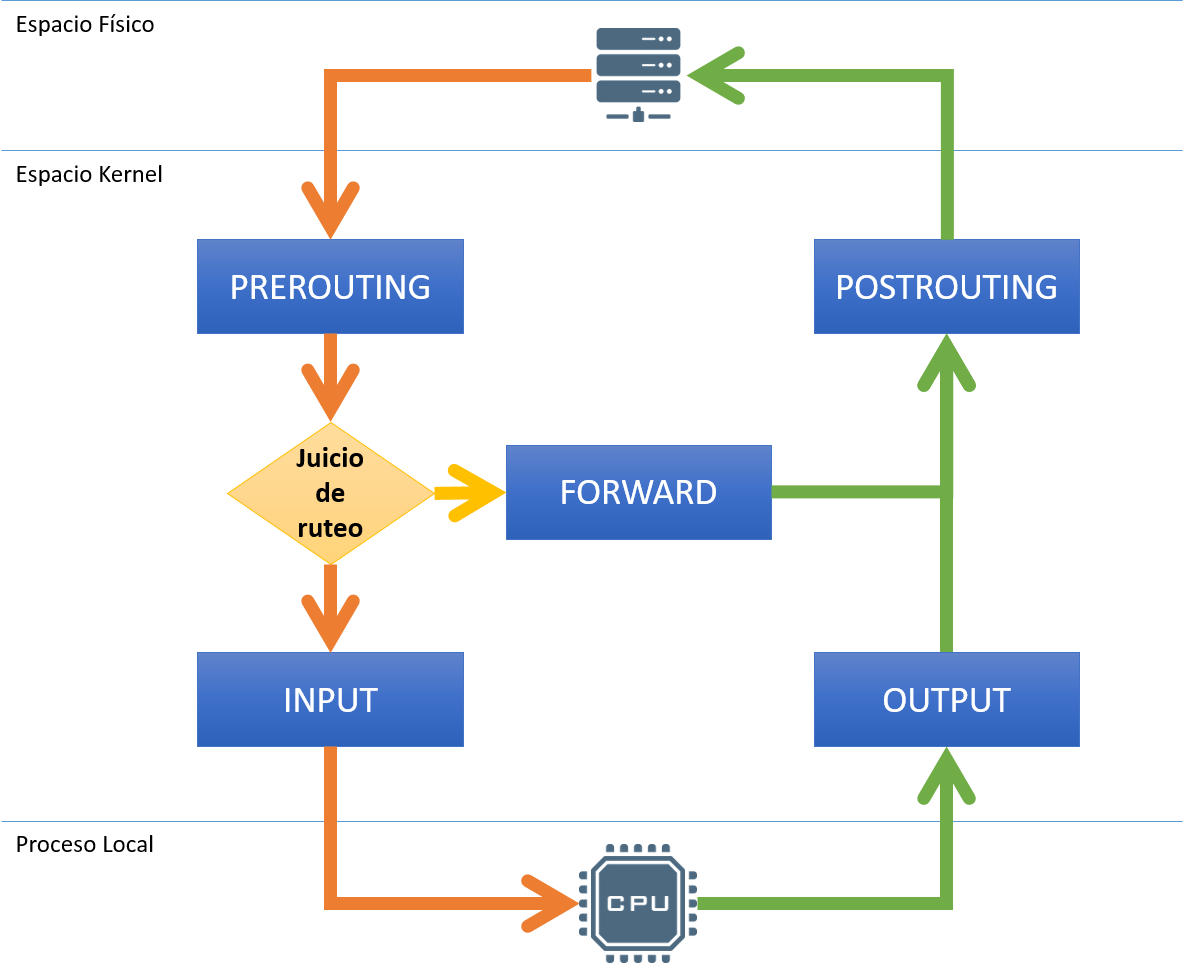
\includegraphics[scale=.3]{imagenes/netfilterArchitecture}
	\caption{Grafico de akamai.}
	\label{netfilterArchitecture}
\end{figure}

Más allá del número de dispositivos o la cantidad --o calidad-- del acceso a Internet, las distintas aplicaciones que ha desarrollado la industria han evolucionado sobre la base de protocolos y sistemas diseñados hace varias décadas, exigiendo siempre la mejor performance posible en pos de garantizar buenos tiempos de respuesta. Los protocolos más celebres de la llamada \emph{familia de protocolos de Internet} son TCP e IP. Sin embargo, son decenas los protocolos y mecanísmos involucrados en las diferentes fases de comunicación entre computadoras y aplicaciones, que permiten en conjunto la operación de la red de redes como hoy la conocemos.

\section{El modelo OSI de conexion en Internet}
La capacidad de conectividad entre 2 distintos dispositivos es resultado del efecto combinado de varias capas de abstracción con responsabilidades divididas. Un diseño de operación que se ilustra en un modelo estándar vigente desde los años 80 es el impulsado por la \emph{Organización Internacional de Normalización} (\textbf{ISO}), mejor conocido como el modelo \textbf{OSI} por sus siglas en inglés \emph{Open System Interconnection}. En la práctica, la importancia de éste modelo radica en servir como una referencia técnica que ilustra los límites en las responsabilidades entre componentes que conforman una arquitectura de interconexión de sistemas.

El modelo OSI reconoce 7 capas de abstracción en el proceso de comunicación entre dispositivos, cada una con obligaciones especificas y que juntas, soportan constructivamente un mecanismo de comunicación estándar para sistemas que por él se rijan. El acierto de éste enfoque está en permitir el desarrollo de soluciones modulares y especificas a cada una de las capas, sin interferir entre capas diferentes y manteniendo así la compatibilidad con aplicaciones que ya operen en capas distintas. Las 7 capas en cuestión se describen a continuación:

\begin{figure}[!h]
	\centering
	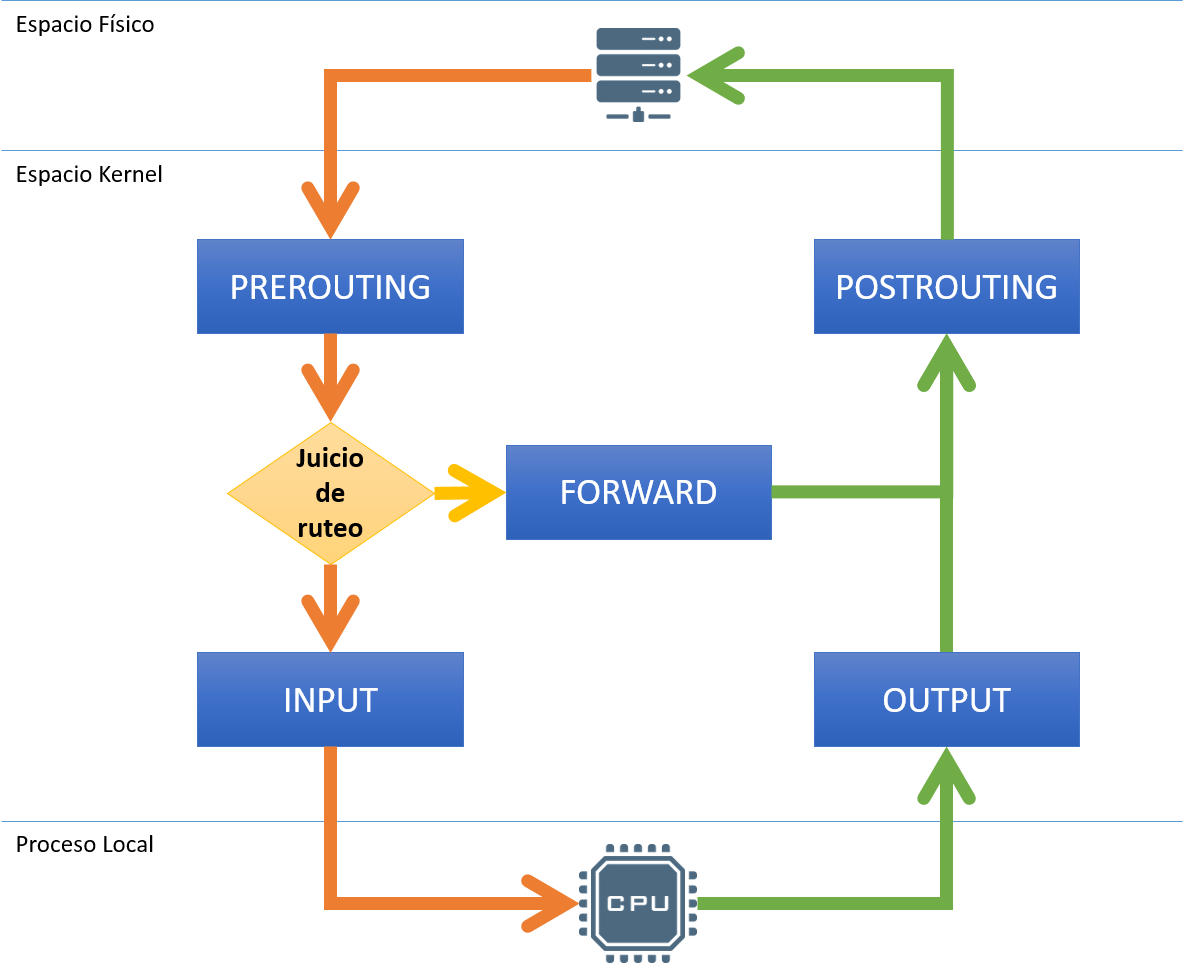
\includegraphics[scale=.3]{imagenes/netfilterArchitecture}
	\caption{Diagrama esquemático de las 7 capas del modelo OSI.}
	\label{netfilterArchitecture}
\end{figure}

\begin{description}
\item[Capa Física] La capa de nivel inferior en el modelo OSI es la capa física. Es ésta capa la responsible de la topología de la red y de la especificación de los medios materiales que consiguen la transmisión de la información, así como también es responsable de la generación real de la comunicación por medio del envío de la información. Es, en definitiva, la encargada del paso a canales físicos de la información a transmitir.

\item[Capa de Enlace] Es la segunda capa del modelo. Ella se encarga de proveer un mecanismo de direccionamiento físico en una máquina que permita el reconocimiento individual de la misma, proveiendo de un primer identificador a las máquinas en el modelo OSI, dado por las direcciones físicas de los dispositivos (\emph{Dirección MAC}). Es responsible también de proveer mecanismos de corrección de errores en el proceso de transmisión de datos que pudiesen manifestarse por problemas de la capa física, haciendo dicha comunicación desde éste punto, confiable.

\item[Capa de Red] Es la tercera capa del modelo. Hace su debut en contextos de multiples equipos interconectados brindando mecanismos de identificación para proveer una capacidad de direccionamiento más amplia con respecto al disponible en las dos primeras capas (que básicamente permitian la comunicación entre un par de máquinas, punto a punto). En éste nivel aparece uno de los protocolos más populares en Internet, el denóminado protocolo IP que supone un mecanismo de identificación único para cada dispositivo en una red, provisto en base a una dirección homónima. Ésta capa establece la capacidad de ruteo en la comunicación como una responsabilidad de los nodos en una infraestructura en red, haciendo cada componente de la red alcanzable para cualquier otro integrante de la misma.

\item[Capa de Transporte] La cuarta capa del modelo, es la que provee de lleno la capacidad de transporte de datos. En éste nivel se incorporan los también celebres protocolos homónimos: TCP (orientado a la conexión) y UDP (orientado a la mensajería). Ésta capa es también responsible de brindar la capacidad de multiplexación a nivel de una máquina, permitiendo la generación de multiples conexiones desde el mismo dispositivo, dicho mecanismo lo consigue al incorporar puertos lógicos de comunicación. De ésta manera, a partir de la capa de Transporte se establece un paradigma base en lo que a programación y esquematización en el area de redes corresponde: La correspondencia sockets \emph{IP:PUERTO}, que conforman finalmente el concepto de tuplas de direccionamiento en el proceso de transporte de datos.

\item[Capa de Sesión] Es la quinta capa del modelo OSI. Tal y como su nombre lo indica su función radica en ser la responsible de mantener un control de sesión en una conexión entre hosts, proveiendo mecanismos de corrección y reconexion en caso de interferencia de una operación entre máquinas. Se encarga de mantener el enlace de comunicación construido en base a las capas inferiores en un proceso de comunicación.

\item[Capa de Presentación] El sexto nivel en el modelo OSI es la capa de presentación, cuya responsabilidad comprende proveer el soporte para dar una correcta interpretación de los datos transmitidos, de manera de conseguir que los datos lleguen de manera reconocible al host de destino. A diferencia de las capas inferiores que se enfocan en los mecanismos de envío de la infromación, ésta capa guarda directa relación con la infromación transmitida y su correcta interpretación.

\item[Capa de Aplicación] Es la última -y de más alto nivel- capa de abstracción del modelo OSI. Es la responsible de proveer una interfaz simple a aplicaciones al acceso a mecanismos de comunicación en red. En otras palabras, es la responsible de proveer el servicio de comunicaciones a las distintas aplicaciones que tengan requerimientos de comunicación.

\end{description}

A pesar de que el modelo OSI plantea responsabilidades delimitadas a cada capa de abstracción, la correspondencia de dicho estándar en la práctica es una labor que queda supeditada a los programadores de sistemas operativos. Finalmente son ellos los que, en mayor o menor medida, hacen corresponder para con el modelo, las implementaciones finales de los módulos de red de un sistema.


\section{Sistemas Operativos Modernos}

\subsection{Interfaces de Comunicación}

\subsection{Sockets en Linux}

\subsection{Mecanismos de Sincronización}

\section{Presentación del Problema}

\subsection{Validación del Problema}

\subsection{Sospechas Iniciales}

\begin{defn}[ver \cite{KAR00}] Definición definitiva $$\frac{d}{dx}\int_a^xf(y)dy=f(x).$$\end{defn}